\RequirePackage[l2tabu, orthodox]{nag}

%\documentclass[final, pdftex, a4paper, 12pt, openbib, ]{article}
\documentclass[final, a4paper, openbib, ]{article}
\usepackage[utf8]{inputenc}
\usepackage[french]{babel}
%\usepackage{fontspec}
%\usepackage{lmodern}
\usepackage[T1]{fontenc}
%\usepackage{graphicx}
\usepackage{alltt}
\usepackage{float}
%\usepackage{times}
%\usepackage{a4wide}
\usepackage{upquote,textcomp}
\usepackage{geometry}
%\usepackage{hyperref}
\usepackage{ulem}
\usepackage[
%pdftex,
final,                      % if you do    want to have clickable-colorful links
pdfstartview = FitV,
linktocpage  = false,       % ToC, LoF, LoT place hyperlink on page number, rather than entry text
breaklinks   = true,        % so long urls are correctly broken across lines
pagebackref  = false,     % add page number in bibliography and link to position in document where cited
]{hyperref}
\usepackage{mathtools}
\geometry{a4paper, portrait, margin=2cm}
%\addtolength{\textheight}{2 cm}
%\addtolength{\oddsidemargin}{-1cm}
%\addtolength{\topmargin}{-1cm}
%\addtolength{\textwidth}{1 cm}

%Good solution for monospaces
%\usepackage{pxfonts} % Or palatino or mathpazo, changes all fonts to something sans
%\usepackage{eulervm} % only changes math fonts, i checked
%\usepackage[ttdefault=true]{AnonymousPro} %Only changes tt fonts
% WHICH ONE TO CHOOSE?
%\usepackage{pslatex}
%\usepackage[ttdefault=true]{AnonymousPro} %Only changes tt fonts
% \usepackage[varg, cmintegrals, cmbraces, ]{newtxtext,newtxmath} % libertine, uprightGreek (U.S.) or slantedGreek (ISO), 
% \usepackage{tgtermes}
% \usepackage{txfonts}
% \usepackage{mathptmx}
% \usepackage[scaled=.90]{helvet}
% \usepackage{courier}
% \usepackage{textcomp}     % required for special glyphs
% \usepackage{bm}   


\usepackage{caption}
\captionsetup[figure]{labelformat=empty}% redefines the caption setup of the figures environment in the beamer class.

%Inconsoloata, a little too light.
%\usepackage{inconsolata}
%\renewcommand{\ttdefault}{Consolas}
%\usepackage{fontspec} %Doesn't work with pdflatex
%\setmonofont{Consolas}

%\renewcommand*\familydefault{\ttdefault} %% Only if the base font of the document is to be typewriter style
%\newcommand\Fontvi{\fontsize{6}{7.2}\selectfont}

%Make tabularx center cells vertically
%\def\tabularxcolumn#1{m{#1}}
%\renewcommand{\tabularxcolumn}[1]{>{\small}m{#1}}

%%Syntax hilighting
%\usepackage{fancyvrb}
\usepackage{minted}
%\usepackage[newfloat]{minted}
\usemintedstyle{borland}
%\usepackage{etoolbox}
%\AtBeginEnvironment{minted}{\singlespacing%
%	\fontsize{14}{14}\selectfont}
%\newminted{java}{fontsize=\footnotesize}
\usepackage{caption}

%\usepackage{multicol}
%\usepackage{vwcol}
%\usepackage{lipsum}
%\usepackage{microtype}
%\setlength{\columnseprule}{0.4pt}
%\renewcommand{\columnseprulecolor}{\color{red}}
\newcommand{\BAD}[1]{{\color{red}#1}}
\newcommand{\GOOD}[1]{{\color{darkgreen}#1}}


\usepackage{graphicx}
\usepackage{colortbl,array}
\usepackage{tabularx}
\definecolor{warningbackground}{RGB}{252,226,158}

\newcommand{\alertwarningbox}[1]{
	\centering
	\begin{tabularx}{0.9\linewidth}{
			>{\columncolor{warningbackground}}c
			>{\columncolor{warningbackground}}X}
		\raisebox{\dimexpr2\baselineskip-\height}
		{
\includegraphics[scale=0.8]{\images/Information.pdf}}&
		\raisebox{\tabcolsep}{\strut}#1\raisebox{-\tabcolsep}{\strut}
	\end{tabularx}
}


\usepackage{xcolor}

%\definecolor{infobackground}{RGB}{217,237,247}
%\definecolor{infoforeground}{RGB}{58,135,173}
%\definecolor{infoborder}{RGB}{188,232,241}

\definecolor{infobackground}{RGB}{217,237,247}
\definecolor{infofrancaisforeground}{RGB}{30,50,70}
\definecolor{infoborder}{RGB}{30,50,70}

\definecolor{infobackground}{RGB}{217,237,247}
\definecolor{infoforeground}{RGB}{30, 80, 150}
\definecolor{infoborder}{RGB}{47, 87, 232}

% ORANGE
\definecolor{infobackground2}{RGB}{255,210,180}
\definecolor{infoforeground2}{RGB}{212, 50, 0}
\definecolor{infoborder2}{RGB}{255, 90, 20}

% GREEN
\definecolor{infobackground3}{RGB}{223,251,223}
\definecolor{infoforeground3}{RGB}{25, 150, 25}
\definecolor{infoborder3}{RGB}{55, 220, 55}


\usepackage{environ}
\usepackage{tikz}
\usetikzlibrary{fit,backgrounds,calc}

\NewEnviron{alertinfo}[1]
{
	\begin{center}
		\begin{tikzpicture}
		\node[inner sep=0pt,
		draw=infoborder,
		line width=1pt,
		fill=infobackground] (box) {\parbox[t]{0.99\textwidth}
			{%
				\begin{minipage}{.12\textwidth}
				\centering\tikz[scale=3]
				\node[scale=1]
				{
					
\includegraphics[scale=0.25]{\images/Information.pdf}
				};
				\end{minipage}%
				\begin{minipage}{.86\textwidth}
				\vskip 10pt
				\textbf{\textcolor{infoforeground}{\large #1}}\par\smallskip
				\textcolor{infoforeground}{\large \BODY}
				\par\smallskip
				\par\smallskip
				\end{minipage}\hfill
			}%
		};
		\end{tikzpicture}
	\end{center}
}


\NewEnviron{alertinfo2}[1]
{
\begin{center}
    \begin{tikzpicture}
    \node[inner sep=0pt,
          draw=infoborder2,
          line width=1pt,
          fill=infobackground2] (box) {\parbox[t]{0.99\textwidth}
        {%
            \begin{minipage}{.12\textwidth}
                \centering\tikz[scale=3]
                \node[scale=1]
                {
                    
\includegraphics[scale=0.25]{\images/Information_orange.pdf}
                };
            \end{minipage}%
           \begin{minipage}{.86\textwidth}
                \vskip 10pt
                \textbf{\textcolor{infoforeground2}{\large #1}}\par\smallskip
                \textcolor{infoforeground2}{\large \BODY}
                \par\smallskip
                \par\smallskip
            \end{minipage}\hfill
        }%
    };
    \end{tikzpicture}
\end{center}
}

\NewEnviron{alertinfo3}[1]
{
\begin{center}
    \begin{tikzpicture}
    \node[inner sep=0pt,
          draw=infoborder3,
          line width=1pt,
          fill=infobackground3] (box) {\parbox[t]{0.99\textwidth}
        {%
            \begin{minipage}{.12\textwidth}
                \centering\tikz[scale=3]
                \node[scale=1]
                {
                    
\includegraphics[scale=0.25]{\images/Information_green.pdf}
                };
            \end{minipage}%
           \begin{minipage}{.86\textwidth}
                \vskip 10pt
                \textbf{\textcolor{infoforeground3}{\large #1}}\par\smallskip
                \textcolor{infoforeground3}{\large \BODY}
                \par\smallskip
                \par\smallskip
            \end{minipage}\hfill
        }%
    };
    \end{tikzpicture}
\end{center}
}

\usepackage{titling}

\newif\ifDRAFT
\DRAFTtrue
% Only comment and uncomment false line :
%\DRAFTfalse

\ifDRAFT
	%Hilighting commands:
	\newcommand{\hl}[1]{\textcolor{green}{#1}}
	\newcommand{\fix}[1]{\textcolor{red}{#1}}	
	\newcommand{\todo}[1]{{\color{red}\bf\em TODO:\/\@#1}}
%	\newcommand{\todo}[1]{{}}	
	\newcommand{\comment}[1]{{\color{blue}\bf\em Comment: \/\@#1}}
%	\newcommand{\comment}[1]{{}}	
	
	\newcommand{\hll}[1]{\textcolor{orange}{\sout{#1}}}
	%\newcommand{\hll}[1]{{}}
	\newcommand{\WR}[1]{\textcolor{purple}{#1}}
\else
	% for final sub
	\newcommand{\hl}[1]{#1}	
	%\newcommand{\hl}[1]{\textcolor{dkgreen}{#1}}
	\newcommand{\fix}[1]{{}}
%	\newcommand{\fix}[1]{\textcolor{red}{#1}}
	\newcommand{\todo}[1]{{}}
	\newcommand{\hll}[1]{{}}
	\newcommand{\comment}[1]{{}}
	\newcommand{\WR}[1]{{#1}}
%	\newcommand{\WR}[1]{\textcolor{purple}{#1}}	
\fi


\newcommand{\codes}{codes}
\newcommand{\images}{images}

%FIX FOR : Undefined control sequence. \tightlist
\providecommand{\tightlist}{%
  \setlength{\itemsep}{0pt}\setlength{\parskip}{0pt}}
  
%\title{GBIAAL 4$^{\mbox{\`eme}}$ année \\ Devoir Surveillé --- Base de données \\ 13 janvier 2016  \\ 1 heure}
\title{GIS 3$^{\mbox{\`eme}}$ année
	%\\TP1 Structures, Listes contiguës, Redirections}
}
\author{\huge \textbf{Introduction à} \\  \Huge\textbf{\texttt{git}}}
\setlength{\parindent}{0pt}
%\pagestyle{empty}
\date{\Large \url{https://rudametw.github.io/teaching/} \\ Polytech Lille}

%\author{Walter Rudametkin}
%\institute[Polytech Lille]{
%Walter.Rudametkin@polytech-lille.fr\\
%\url{https://rudametw.github.io/teaching/}\\
%\vspace{0.5cm}Bureau F011\\
%Polytech Lille\\

\begin{document}
%\vspace{-15cm}
\vspace{-5cm}
\posttitle{\par\end{center}}
\setlength{\droptitle}{-45pt}
\maketitle
%\thispagestyle{empty}

\section{Objectifs}\label{objectifs}

\begin{itemize}
\item Apprendre à se servir d'un Logiciel de Gestion de Version\footnote{\url{https://fr.wikipedia.org/wiki/Logiciel_de_gestion_de_versions}}.
\item Maîtrisez le versionnement d'un projet logiciel.
\item Partager un projet et travailler en équipe.
\end{itemize}

\begin{alertinfo}{IMPORTANT !}
Lisez attentivement la sortie de \textbf{\textit{chaque}} commande \texttt{git}.
Il est fortement conseillé de travailler exclusivement sur terminal pour ce TP.
\end{alertinfo}

\section{Contexte et préparation}
\label{context} 

\subsection{Configuration de \texttt{bash}}

\paragraph{\texttt{.bashrc} et \texttt{gitprompt.sh}}
Pour commencer ce TP, nous vous fournissons une configuration avancée de \texttt{bash} (l'interpréteur en ligne de commande utilisé par défaut).
Vous pouvez lancer, une seule fois par compte, la commande suivante qui aura pour objectif de mettre à jour votre fichier \texttt{~/.bashrc} et d'installer \texttt{gitprompt.sh} sur vos comptes.
\begin{minted}[mathescape=true,escapeinside=||,tabsize=4
%	,fontsize=\footnotesize,
]{bash}
	~wrudamet/public/set_bashrc.sh
\end{minted}

Pour les curieux, vous pouvez regarder vos fichiers \mintinline{bash}{~/.bashrc}, \mintinline{bash}{~/.bashrc-students} et \mintinline{bash}{~/git-prompt.sh} pour comprendre ce qui a été ajouté.
N'hésitez pas à éditer ou supprimer les changements si vous préférez.


\paragraph{Terminals}
%\WR{Copier le fichier XXX.aide pour récupèrer quelques commandes. }
Nous vous proposons de travailler sur plusieurs terminals ouverts simultanément, une disposition possible est indiquée dans la figure~\ref{terminals} mais vous pouvez les ranger à votre convenance tout au longue du TP.
\begin{figure}[h]
	\centering
	{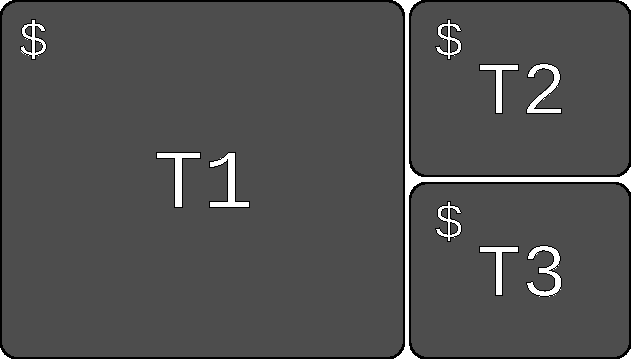
\includegraphics[scale=0.4]{images/terminals.pdf}}
	\caption{Figure 1: Disposition des terminals proposée.}
	\label{terminals}
\end{figure}

Cette disposition vous permettra d'exécuter vos commandes \texttt{git} dans le terminal \texttt{T1}, tout en exécutant des commandes de \textit{suivi} dans les terminaux \texttt{T2} et \texttt{T3}.\\

Dans un premier temps, positionnez \texttt{T1}, \texttt{T2} et \texttt{T3} dans le répertoire où vous allez travailler via la commande \texttt{cd}.\\

La commande \texttt{watch}\footnote{\url{https://en.wikipedia.org/wiki/Watch\_(Unix)}} permet de répéter une commande toute les $X$ secondes. Dans le terminal \texttt{T2} exécutez :
\begin{minted}[mathescape=true,escapeinside=||,tabsize=4
%	,fontsize=\footnotesize,
]{bash}
	watch -d -n3 tree -a tpgit
\end{minted}

Et dans le terminal \texttt{T3} exécutez :
\begin{minted}[mathescape=true,escapeinside=||,tabsize=4
%	,fontsize=\footnotesize,
]{bash}
	watch cat ~/.gitconfig
\end{minted}

Il est normal que ces commandes affichent pour le moment des erreurs car nous n'avons pas encore créé le répertoire \texttt{tpgit} ni le fichier \texttt{.gitconfig}.


\subsection{Configuration de votre compte \texttt{git}}

Dans un projet gérer à plusieurs, il est important de savoir qui a fait quoi. \texttt{git} a donc besoin d'une configuration pour identifier vos futurs \emph{commits}, et vous pouvez également spécifier certains comportements.
Les commandes suivantes vont modifier votre fichier \texttt{.gitconfig}, tapez les une à une en regardant les changements dans le terminal \texttt{T3}:

\begin{minted}[mathescape=true,escapeinside=||,tabsize=4
%	,fontsize=\footnotesize,
]{bash}
	git config |-{}-|global user.name "votre nom"
	git config |-{}-|global user.email nom.prenom@polytech-lille.net
	git config |-{}-|global core.editor kate
	git config |-{}-|global push.default simple
	git config |-{}-|global color.decorate full
	git config |-{}-|global merge.conflictstyle diff3
\end{minted}

Si vous préférez un autre éditeur à la place de \texttt{kate}, vous pouvez l'utiliser (e.g., \texttt{nano}, \texttt{vim}, \texttt{emacs}, \texttt{gedit}).

\begin{alertinfo}{Rappel !}
Les configurations de \texttt{git} et de \texttt{bash} doivent se faire une fois pour chaque compte.
Votre binôme devra réaliser la même configuration sur son compte, et si vous comptez travailler sur un autre PC, il faudra récupérer votre fichier \texttt{.gitconfig} ou relancer les commandes de configuration.
\end{alertinfo}

\section{Initialisation d'un dépôt \texttt{git}}

Nous allons travailler sur un projet qu'on appellera \texttt{tpgit}.
En vous aidant des supports du cours (slide 13), vous devez :
\begin{itemize}
\item créer un répertoire \texttt{tpgit}
\item initialiser dans ce répertoire un dépôt git vide
\item regarder les fichiers créés pour ce dépôt, ils seront affichés dans le terminal \texttt{T2}
\item créer un fichier \texttt{fruits.txt}
\item réaliser un commit en ajoutant 2 fruits à \texttt{fruits.txt}.
Pour rappel, l'enchaînement des commandes est : \mintinline{bash}{status, add, status, commit, status, log}.
Lisez la sortie de chaque commande pour comprendre leur fonctionnement.
\item réaliser 3 commits de plus en ajoutant à chaque fois des fruits.
\end{itemize}

\begin{alertinfo3}{Astuce !}
Utilisez les commandes \texttt{git status}, \texttt{git diff \textit{nom\_fichier}} et \texttt{git log} pour comprendre l'état de votre dépôt. La commande \texttt{git log -}\texttt{-graph -}\texttt{-oneline -}\texttt{-decorate -}\texttt{-all} vous donne une historique détaillé avec toutes les branches, étiquettes et commits.
Pour quoi ne pas la garder à la vu dans le terminal \texttt{T3} (l'éxécuter avec un \texttt{watch -d -n5 git log \ldots}) ?
\end{alertinfo3}


\section{Branches \texttt{git}}

Branches \texttt{legumes}
\begin{itemize}
\item créer une branche \texttt{legumes}
\item ajouter un fichier \texttt{legumes.txt} sur cette branche
\item réaliser 3 commits différents en ajoutant des légumes à \texttt{legumes.txt}
\item vérifier l'historique de vos commits à l'aide de \texttt{git log}.
\end{itemize}

Branches \texttt{sauces}
\begin{itemize}
\item créer une branche \texttt{sauces}
\item ajouter un fichier \texttt{sauces.txt} sur cette branche
\item réaliser 2 commits différents
\item vérifier l'historique de vos commits et l'existence de \textbf{3 branches} (master, legumes, sauces) à l'aide de \texttt{git branch} et \texttt{git log}.
\end{itemize}


\section{Merges \texttt{git}}
Vous avez décidé que vos commits dans les branches \texttt{legumes} et \texttt{sauces} sont pertinents, maintenant vous devez les intégrer dans \texttt{master}.
\begin{itemize}
\item aller sur la branche \texttt{legumes}
\item vérifier l'état de votre espace de travail (e.g., l'inexistence du fichier \texttt{sauces.txt})
\item merger \texttt{master} dans \texttt{legumes}
\item si tout c'est bien passé, merger \texttt{legumes} dans \texttt{master}
\item vérifier l'historique de vos commits et l'apparition de \texttt{legumes.txt} sur la branche \texttt{master}\\
\end{itemize}

Vous pouvez maintenant merger la branche \texttt{sauces} avec \texttt{master} en suivant le même processus.
Vérifiez que tous les branches sont à jour.

\section{Dépôt distant}

Nous allons activer vos comptes sur le serveur GitLab de Polytech et créer un dépôt vide où vous allez pousser votre dépôt existant \texttt{tpgit}.
GitLab vous permet de gérer votre projet et fourni plusieurs fonctionnalités intéressantes (e.g., issues, graphes, édition de fichiers, recherche de contributeurs, dashboard).\\

Vous devez :
\begin{itemize}
\item Connectez-vous sur \url{https://archives.plil.fr/}
\item Créez un projet sur le serveur GitLab de Polytech
\item Poussez votre dépôt \texttt{tpgit} sur le GitLab
\item Ajoutez votre binôme aux membres de votre projet avec le niveau de droit \textit{Developer} (il devra se connecter une première fois avant d'apparaître dans la liste des membres)
\end{itemize}

\paragraph{Créer un dépôt sur GitLab et poussez \texttt{tpgit}}
\begin{enumerate}
\item Cliquer sur \textit{+New Projet} en haut pour créer un nouveau projet
\item Donner un nom à votre projet et cliquer sur \textit{Create project}
\item Vous êtes emmenés dans votre projet, qui est vide, avec les instructions des différentes formes d'initialisation.
Lisez les propositions.
Vous devez \textbf{impérativement changer l'url de \texttt{SSH} à \texttt{HTTPS}}
\item Retrouvez les instructions \textit{Push an existing Git repository}. Vous allez copier et exécuter la commande :\\ \texttt{git remote add origin https://archives.plil.fr/<user>/<project.git>} avec le bon url\\ suivi de \texttt{git remote -v}, et \texttt{git push -u origin master}
\item Rafraîchissez la page de votre projet GitLab, votre projet \texttt{tpgit} doit s'y retrouver
\item Naviguez votre projet sur Gitlab pour voir l'historique de commits, vos fichiers, vos graphes, etc.
\end{enumerate}	

\begin{alertinfo2}{Attention !}
Il y a deux protocoles réseau pour échanger avec GitLab, HTTPS et SSH. Nous vous conseillons de travailler avec HTTPS dans un premier temps.
Dans le futur vous pouvez choisir SSH, qui est plus puissant et flexible, mais il faudra configurer vos clés privés et publiques en suivant l'aide \url{https://archives.plil.fr/help/ssh/README}
\end{alertinfo2}


\paragraph{Gestion des membres de votre projet}
\begin{enumerate}
\item Aller dans les \textit{Settings} de votre projet (menu à gauche),
\item Cliquer sur \textit{Members} dans le menu \textit{Settings} (menu à gauche),
\item Cliquer sur \textit{New project member} en haut à droite,
\item Chercher le login de la personne que vous voulez ajouter (votre binôme),
\item Sélectionner le niveau de droit de cette personne (\textit{Developer}),
\item Cliquer sur \textit{Add users}.
\end{enumerate}


\section{Travail collaboratif}

Votre binôme devra se mettre à travailler avec vous.
Après avoir configuré son compte (section \ref{context}) il devra :
\begin{itemize}
\item Se connecter sur votre projet dans GitLab \url{https://archives.plil.fr/<login>/<projet.git>}
\item Cliquer sur HTTPS
\item Cloner le projet à l'aide de la commande \texttt{git clone <url>}
\item Regardez l'historique du projet.
\end{itemize}

\section{Travail simultané}

Vous allez travailler en même temps sur votre projet, chacun sur son propre dépôt local, et vous allez synchroniser les changements après.

\subsection{Merge sans conflit}

\paragraph{Travail de Binôme1}
\begin{itemize}
\item créer une branche \texttt{epices}
\item ajouter un fichier \texttt{epices.txt} sur cette branche
\item réaliser 2 commits différents
\item merger vos commits dans \texttt{master}
\item récupérer les changements sur le serveur (\texttt{git pull})
\item pousser vos changements vers le serveur GitLab à l'aide de la commande \texttt{git push}
\end{itemize}

\paragraph{Travail de Binôme2}
\begin{itemize}
\item créer une branche \texttt{herbes}
\item ajouter un fichier \texttt{herbes.txt} sur cette branche
\item réaliser 2 commits différents
\item merger votre branche dans \texttt{master}
\item récupérer les changements sur le serveur (\texttt{git pull})
\item pousser vos changements vers le serveur GitLab à l'aide de la commande \texttt{git push}\\
\end{itemize}

\paragraph{Tous les deux}
\begin{itemize}
\item vérifier l'existence des fichiers \texttt{epices.txt} et \texttt{herbes.txt} dans vos deux dépôts
\item vérifier l'historique des deux dépôts... est-ce que tous les ID de commits sont les mêmes ? Vous avez trouvé le dernier commit de merge ? Vous voyez les commits de votre binôme ?\\
\end{itemize}

Un de vous deux a été le premier à pousser, et l'autre a dû merger les changements avant de pouvoir pousser son travail.
Parce que vous avez travaillé sur des fichiers différents, le merge a été résolu automatiquement.
Nous allons maintenant vous obliger à générer des conflits et à les résoudre.

\begin{alertinfo3}{Astuce !}
Vous en avez marre de taper votre login et mot de passe à chaque \texttt{pull} et \texttt{push} ?
Git peut se souvenir de votre identité pendent un temps déterminé, par exemple, pour une heure utilisez la commande :\\
\texttt{git config -{}-global credential.helper 'cache -{}-timeout=3600'}
\end{alertinfo3}


\subsection{Merge avec conflit}

\paragraph{Générer un conflit}
\begin{itemize}
\item éditez tous les deux, chacun sur son dépôt, le fichier \texttt{fruits.txt}, de façon à \textbf{effacer} certains fruits et à \textbf{ajouter} des nouveaux (faites des changements différents)
\item commitez vos changements mais ne poussez pas encore
\item binôme1 pousse ses changements en premier
\item binôme2 pull les changements de binôme1 et\ldots CONFLIT !
\item \texttt{git status}, lisez la sortie
\item à l'aide du cours (slides 26-28), essayez de résoudre ce conflit
\item une fois résolu, merger vos changements et poussez vers le serveur
\item binome1, récupérez les changements et vérifiez l'état de \texttt{fruits.txt}
\end{itemize}

\paragraph{Générer un 2ème conflit, inverser les rôles}
\begin{itemize}
\item comme précédemment, générer un conflit dans le fichier \texttt{legumes.txt} mais cette fois inversez les rôles :  binome2 pousse en premier, binome1 résout le conflit.
\item au moment du conflit, c'est-à-dire, tout de suite après un \texttt{git pull} ou \texttt{git merge}, vous pouvez annuler le merge avec la commande \texttt{git merge -{}-abort}.
Essayez la commande et vérifier que votre dépôt revient dans l'état avant le \texttt{pull} (plus de conflits, vérifier avec \texttt{status}).
Refaite \texttt{git pull} et vous allez retrouver le conflit, résolvez-le cette fois.
\end{itemize}

\begin{alertinfo3}{Astuce !}
Pour minimiser les conflits, il faut s'assurer que tout le monde maintienne son dépôt à jour.
Il faut régulièrement merger vers la branche \texttt{master}, faire \texttt{git pull} sur vos branches, et corriger les éventuels petits conflits quand ils sont simples.
Avant de pousser vos changements avec \texttt{git push}, il faut toujours faire un \texttt{git pull}.
\end{alertinfo3}

\section{Documenter votre projet à l'aide de Markdown}

Markdown est un langage de balisage léger, plus rapide à écrire que HTML et très flexible.
Il est interprété automatiquement par GitLab (et plein d'autres produits) et permet de documenter votre projet ou même d'écrire vos rapports.\\

Créez un fichier \texttt{README.md} à la racine de votre dépôt en utilisant la syntaxe markdown pour spécifier des titres, listes, des extraits de code.
Vous devez au minimum :
%\begin{itemize}
	\begin{itemize}
	\item donnez une description de votre projet
	\item listez les auteurs dans une section \textit{Auteurs}
	\item listez les objectifs dans une section \textit{Objectifs}\\
	\end{itemize}
%\end{itemize}

Vous pouvez vous inspirer de cet exemple sur Github :\\
\url{https://gist.github.com/PurpleBooth/109311bb0361f32d87a2}\\
(cliquer sur RAW pour avoir les sources).
Vérifiez que votre README s'affiche correctement sur GitLab.
%\url{https://gist.githubusercontent.com/PurpleBooth/109311bb0361f32d87a2/raw/824da51d0763e6855c338cc8107b2ff890e7dd43/README-Template.md}



\section{Continuer à apprendre}

Si vous voulez maitriser \texttt{git}, n'hésitez pas à faire le tutoriel donné par le laboratoire CRIStAL de l'université de Lille.
Il y a beaucoup de fonctionnalités avancées qui peuvent s'avérer très utiles.
\url{http://www.cristal.univ-lille.fr/TPGIT/} .\\

Vous pouvez également consulter les liens suivants :
\paragraph{Liens, aides et outils}
\begin{itemize}
	\item Où stocker vos projets
	\begin{itemize}
		\item \url{https://archives.plil.fr/}
		\item \url{https://github.com/}
		\item \url{https://bitbucket.org/}
		\item Votre serveur perso (e.g., installer GitLab chez vous)
	\end{itemize}
	\item Tutoriels
	\begin{itemize}
		\item \url{http://www.cristal.univ-lille.fr/TPGIT/}
		\item \url{https://crypto.stanford.edu/~blynn/gitmagic/intl/fr/book.pdf}
		\item \url{https://learngitbranching.js.org/}
		\item \url{https://try.github.io/}
		\item \url{https://git-scm.com/book/fr/v2}
	\end{itemize}
	\item Vidéos
	\begin{itemize}
		\item \url{https://www.youtube.com/watch?v=OqmSzXDrJBk}
		\item \url{https://www.youtube.com/watch?v=uR6G2v_WsRA}
		\item \url{https://www.youtube.com/watch?v=3a2x1iJFJWc}
		\item \url{https://www.youtube.com/watch?v=1ffBJ4sVUb4}
		\item \url{https://www.youtube.com/watch?v=duqBHik7nRo}
	\end{itemize}
\end{itemize}
\end{document}